\subsection{Imaging in LM and N}
\label{ssec:overview_lm_imaging}

% HB 20230731: This note is not really necessary I think.
%\textbf{Note: The pipeline layout has been modified compared to the
%  PDR design in order to achieve better modularity. Basic reduction
%  and background subtraction have been split into two recipes that now
%  are applied to both standard calibration and science data. ADI recipes have been added since PDR however integration of \ac{HCI}
%  into this workflow requires more work: \ac{HCI} images will be treated
%  the same way at least through basic reduction, possibly through
%  background subtraction. \ac{ADI} combination may require a separate
%  recipe, at least for some \ac{HCI} configurations.}

The purpose of the pipeline is to correct or remove contributions from
the instrument, telescope, and atmosphere and produce science-grade
data products.  In the case of the METIS imaging modes the main
contributions to correct or remove are dark current, flatfield, bad
pixels, and, most importantly, thermal background emission from the
sky and the telescope. Further effects include persistence,
cross-talk, geometric distortions, etc. The final product of the
imaging pipeline is one or more image(s) that are flux-calibrated in units of
photons/s/pixel against a standard star.
Several images can be stacked into a single possibly mosaiced image.

Due to the differences in characteristics between the HAWAII2RG
detector used for imaging in the L and M bands and the GeoSnap
detector used for the N band, the operational concept for the two
imager subsystems are quite different. This induces differences in the
way the data have to be reduced.

The GeoSnap detector has more stable gain than AQUARIUS detector,
which was still in the baseline at PDR\@.  Chopping is still necessary, albeit
at a lower frequency of a few Hz, and a chop/nod technique, which meets the
specific ELT requirements (Section~\ref{sssec:nbandsbackgroundsubtracion}),
will be employed  for background subtraction.  As the dark
signal is automatically removed when the exposures from the different
chop and nod positions are combined no master dark is required for the
reduction of science data. The GeoSnap data is also flat fielded.

Observations and reduction of LM band data with the HAWAII2RG detector
can proceed as in the near infrared. After dark subtraction and
flat-fielding, the background is estimated from a series of dithered
science exposures or from exposures on a nearby blank patch of sky.

The association maps for the current designs of the imaging pipelines
in~LM and~N are shown in Figs.~\ref{fig:IMG_LM_Assomap}
and~\ref{fig:IMG_N_Assomap}, respectively.

%\TODO{For \ac{HCI} data, \ac{ADI} may need to be part of reduction recipe if
%  individual background subtracted images are the goal?} We provide ADI recipes since PDR.

\begin{landscape}
  \begin{figure}
    \centering
    \resizebox{\linewidth}{!}{%% IMG_LM_assomap_tikz.tex
%% Created by Oliver Czoske
%%
%% 2019-02-26: Changed to LM only
%% 2019-02-26: Try to align it with the recipe flow
%% 2020-09-07: Pipeline redesign

\sffamily


% ADDING NEW DEFINITIONS -------------------------------------------- start
\definecolor{listingbg}{gray}{0.95}
\definecolor{darkgreen}{rgb}{0.0, 0.7, 0.0}
\definecolor{darkblue} {rgb}{0.0, 0.0, 0.7}
\definecolor{cyan} {rgb}{0.0, 0.4, 0.4}
\definecolor{darkred}  {rgb}{0.7, 0.0, 0.0}
\definecolor{darkorange}{rgb}{1.0, 0.49, 0.0}
\definecolor{violett}{rgb}{255, 0, 255}
\definecolor{turq}{rgb}{0.0, 0.7, 0.8}
\definecolor{fits}{rgb}{0.4, 0.1, 1}


\makeatletter
\lstdefinestyle{RAWstyle}{%
  basicstyle=\ttfamily\color{black}%
  \lst@ifdisplaystyle\scriptsize\fi}

\lstdefinestyle{PARstyle}{%
  basicstyle=\ttfamily\color{black}%
  \lst@ifdisplaystyle\scriptsize\fi}

\lstdefinestyle{DRLstyle}{%
  basicstyle=\ttfamily\color{black}%
  \lst@ifdisplaystyle\scriptsize\fi}

\lstdefinestyle{RECstyle}{%
  basicstyle=\ttfamily\color{black}%
  \lst@ifdisplaystyle\scriptsize\fi}

\lstdefinestyle{QCstyle}{%
  basicstyle=\ttfamily\color{black}%
  \lst@ifdisplaystyle\scriptsize\fi}

\lstdefinestyle{TPLstyle}{%
  basicstyle=\ttfamily\color{black}%
  \lst@ifdisplaystyle\scriptsize\fi}

\lstdefinestyle{PRODstyle}{%
  basicstyle=\ttfamily\color{black}%
  \lst@ifdisplaystyle\scriptsize\fi}

\lstdefinestyle{EXTCALIBstyle}{%
  basicstyle=\ttfamily\color{black}%
  \lst@ifdisplaystyle\scriptsize\fi}

\lstdefinestyle{STATCALIBstyle}{%
  basicstyle=\ttfamily\color{black}%
  \lst@ifdisplaystyle\scriptsize\fi}
\makeatother

%%% This file contains definitions of shapes and nodes used
%%% for a recipe workflow
%%% Author       : Oliver Czoske
%%% Created      : 2021-03-03
%%% Last Changed : 2021-03-03
%%% Changes:
%%%

\usetikzlibrary{
  shapes.misc,
  positioning,
  calc,
  arrows.meta}

%% All connecting lines have an arrow
\tikzset{
  connection_arrow/.style={->, >=Latex[open], thick}
}

%% Start and stop buttons (black disks, stop with ring)
%% These are pics, use as
%%         \pic (name) [above of=..] {picname};
\tikzset{
  start/.pic = {
    \node (-m) at (0, 0){};
    \filldraw [fill=black] (0, 0) circle (0.2);
  }
}

\tikzset{
  stop/.pic = {
    \node (-m) at (0, 0){};
    \node (-t) at (0, -0.3){};
    \filldraw [fill=black] (0, 0) circle(0.2);
    \draw[black] (0, 0) circle (0.3);
  }
}


%%%% Various boxes and their colours
%%%% These are nodes, use as
%%%% \node (name) [type, location]  {text};

\definecolor{stepcolor}{RGB}{210,169,188}
\definecolor{rawcolor}{RGB}{205,205,205}
\definecolor{externalcolor}{RGB}{183,255,255}
\definecolor{calibcolor}{RGB}{255,250,216}
\definecolor{calproductcolor}{RGB}{185,184,237}
\definecolor{qcproductcolor}{RGB}{255,201,165}
\definecolor{sciproductcolor}{RGB}{197,219,183}
\definecolor{framecolor}{RGB}{127,13,65}

\tikzset{
  %% template : the template(s) that trigger(s) the recipe
  template/.style={
    rectangle,
    draw=black,
    minimum width=4.0cm,
    minimum height=0.5cm,
    align=center
  },
  %% input : the input files
  input/.style={
    rectangle,
    fill=rawcolor,
    minimum width=4.0cm,
    minimum height=0.75cm,
%     text width=3cm,
    align=center
  },
  %% calib : calibration input
  calib/.style={
    rectangle,
    fill=calibcolor,
    minimum width=4.0cm,
    minimum height=0.75cm,
%     text width=3cm,
    align=center
  },
  %% external : external input
  external/.style={
    rectangle,
    fill=externalcolor,
    minimum width=4.0cm,
    minimum height=0.75cm,
%     text width=3.5cm,
    align=center
  },
  %% params : parameters
  params/.style={
    rectangle,
    draw=red,
    thick,
    minimum width=4.0cm,
    minimum height=0.75cm,
%     text width=3cm,
    align=center
  },
  %% redstep : a reduction step
  %%      ("step" is predefined and can't be used)
  redstep/.style={
    rectangle,
    rounded corners=0.2cm,
    fill=stepcolor,   %%% define colour!
    minimum width=4.0cm,
    minimum height=1cm,
%     text width=3cm,
    align=center
  },
  %% connection : connection to input or output
  connection/.style={
    circle,
    fill=black,
    minimum size=0.15cm,
    inner sep=0pt
  },
  %% sciproduct : a science product
  sciproduct/.style={
    rectangle,
    fill=sciproductcolor,
    minimum width=4.0cm,
    minimum height=0.75cm,
%     text width=3.5cm,
    align=center
  },
  %% calproduct : a calibration product
  calproduct/.style={
    rectangle,
    fill=calproductcolor,
    minimum width=4.0cm,
    minimum height=0.75cm,
%     text width=3.5cm,
    align=center
  },
  %% frame : frame around the recipe
  %% This is a path, use as
  %%    \draw [frame] (upper left) rectangle (lower right);
  frame/.style={framecolor, very thick, dashed}
}


%%% Picture: flow chart
\begin{tikzpicture}[on grid=false,node distance=0.8cm]

  \matrix (recipes) [column sep=0.1cm, row sep=1cm]{
    % The matrix has colums
    % detlin_*, dark_*, flat_*, std_*, sci1_*, sci2_*, adi
    %
    % The matrix has rows
    % *_raw, *_dark, *_flat, *_std, *_sci1, *_sci2, *_prod

    % Row *_raw
    \node [above] (lin_raw){%
      \recipebox{DETLIN}{det\_lingain}
    };
    &
    \node [above] (pers_raw){%
        \recipebox{PERSISTENCE}{persistence\_map}
    };
    &
    \node [above] (dist_raw){%
      \recipebox{DISTORTION}{lm\_img\_distortion}
    };
    &
    \node[above] (dark_raw) {%
      \recipebox{DARK}{det\_dark}
    };
    &
    \node[above] (flat_raw){%
      \recipebox{FLAT}{lm\_img\_flat}
    };
    &
    \node[above] (all1_raw){%
      \recipebox{SCIENCE, STD}{lm\_img\_basic}
    };
    &
    \node[above] (all2_raw){%
      \recipebox{SCIENCE, STD}{lm\_img\_background}
    };
    &
    \node[above] (std_raw){%
      \recipebox{PHOT STD}{lm\_img\_std\_process}
    };
    &
    \node[above] (sci1_raw){%
      \recipebox{SCIENCE}{lm\_img\_sci\_calibrate}
    };
    &
    \node[above] (sci2_raw){%
      \recipebox{SCIENCE}{lm\_img\_sci\_coadd}
    };

   % \node[above] (sci2_raw){%     % needs width parameter to box
   %  \begin{tcolorbox}[%
   %    width=4.5cm,
   %    colback=recipecolor]
   %    \centering lm\_img\_sci\_postprocess
   %  \end{tcolorbox}};
   %&
   %\node[above] (adi_raw){%
   %  \recipenotitlebox{adi\_postprocess}
   %};
   \\

    %%% Calibration products
    % Row *_lin
    \node (lin_lin) [statcalfile]{\hyperref[dataitem:linearity_2rg]{\STATCALIB{LINEARITY_2RG}}}; &
    \node (pers_lin)[empty]{}; &
    \node (dist_lin)[empty]{}; &
    \node (dark_lin)[empty]{}; &
    \node (flat_lin)[connection]{}; &
    \node (all1_lin)[connection]{}; &
    \node (all2_lin)[empty]{}; &
    \node (std_lin)[empty]{}; &
    \node (sci1_lin)[empty]{}; &
    \node (sci2_lin)[empty]{}; \\

    % Row persistence
    \node (lin_pers)[empty]{}; &
    \node (pers_pers)[extcalfile]{\STATCALIB{PERSISTENCE_MAP}}; &
    \node (dist_pers)[empty]{}; &
    \node (dark_pers)[empty]{}; &
    \node (flat_pers)[connection]{}; &
    \node (all1_pers)[connection]{}; &
    \node (all2_pers)[empty]{}; &
    \node (std_pers)[empty]{}; &
    \node (sci1_pers)[empty]{}; &
    \node (sci2_pers)[empty]{}; \\

    % Row *_dark
    \node (lin_dark) [empty]{}; &
    \node (pers_dark) [empty]{}; &
    \node (dist_dark) [empty]{}; &
    \node (dark_dark) [calibproduct]{\hyperref[dataitem:master_dark_2rg]{\PROD{MASTER_DARK_2RG}}}; &
    \node (flat_dark)[connection]{}; &
    \node (all1_dark)[connection]{}; &
    \node (all2_dark)[empty]{}; &
    \node (std_dark)[empty]{}; &
    \node (sci1_dark)[empty]{}; &
    \node (sci2_dark) [empty]{}; \\

    % Row *_flat
    \node (lin_flat) [empty]{}; &
    \node (pers_flat) [empty]{}; &
    \node (dist_flat)[empty]{}; &
    \node (dark_flat)[empty]{}; &
    \node (flat_flat) [calibproduct]{\hyperref[dataitem:master_flat_2rg]{\PROD{MASTER_FLAT_2RG}}}; &
    \node (all1_flat)[connection]{}; &
    \node (all2_flat)[empty]{}; &
    \node (std_flat)[empty]{}; &
    \node (sci1_flat)[empty]{}; &
    \node (sci2_flat) [empty]{}; \\

    % Row *_all1
    \node (lin_all1)[empty]{}; &
    \node (pers_all1) [empty]{}; &
    \node (dist_all1)[empty]{}; &
    \node (dark_all1)[empty]{}; &
    \node (flat_all1)[empty]{}; &
    \node (all1_all1)[calibproduct]{\hyperref[dataitem:std_reduced]{\PROD{STD_REDUCED}}}; &
    \node (all2_all1)[calibproduct]{\hyperref[dataitem:std_bkg_sub]{\PROD{STD_BKG_SUB}}}; &
    \node (std_all1)[connection]{}; &
    \node (sci1_all1)[empty]{}; &
    \node (sci2_all1) [empty]{}; \\

% Row *_all2
    \node (lin_all2) [empty]{}; &
    \node (pers_all2) [empty]{}; &
    \node (dist_all2)[empty]{}; &
    \node (dark_all2)[empty]{}; &
    \node (flat_all2)[empty]{}; &
    \node (all1_all2)[scienceproduct]{\hyperref[dataitem:sci_reduced]{\PROD{SCI_REDUCED}}}; &
    \node (all2_all2)[scienceproduct]{\hyperref[dataitem:sci_bkg_sub]{\PROD{SCI_BKG_SUB}}}; &
    \node (std_all2)[empty]{}; &
    \node (sci1_all2)[connection]{}; &
    \node (sci2_all2) [empty]{}; \\

    % Row *_dist
    \node (lin_dist) [empty]{}; &
    \node (pers_dist) [empty]{}; &
    \node (dist_dist)[statcalfile]{\hyperref[dataitem:distortion_tab]{\STATCALIB{DISTORTION_TAB}}}; &
    \node (dark_dist)[empty]{}; &
    \node (flat_dist) [empty]{}; &
    \node (all1_dist)[empty]{}; &
    \node (all2_dist)[empty]{}; &
    \node (std_dist)[empty]{}; &
    \node (sci1_dist)[connection]{}; &
    \node (sci2_dist) [empty]{}; \\

    % Row *_std
    \node (lin_std) [empty]{}; &
    \node (pers_std) [empty]{}; &
    \node (dist_std)[empty]{}; &
    \node (dark_std)[extcalfile]{\hyperref[dataitem:fluxstd_catalog]{\EXTCALIB{FLUXSTD_CATALOG}}}; &
    \node (flat_std)[empty]{}; &
    \node (all1_std)[empty]{}; &
    \node (all2_std)[empty]{}; &
    \node (std_std)[connection]{}; &
    \node (sci1_std)[empty]{}; &
    \node (sci2_std) [empty]{}; \\

    % Row *_sci1
    \node (lin_sci1) [empty]{}; &
    \node (pers_sci1) [empty]{}; &
    \node (dist_sci1)[empty]{}; &
    \node (dark_sci1)[empty]{}; &
    \node (flat_sci1)[empty]{}; &
    \node (all1_sci1)[empty]{}; &
    \node (all2_sci1)[empty]{}; &
    \node (std_sci1)[calibproduct]{\hyperref[dataitem:fluxcal_tab]{\PROD{FLUXCAL_TAB}}}; &
    \node (sci1_sci1)[connection]{}; &
    \node (sci2_sci1)[empty]{}; \\

    % Row *_sci2
    \node (lin_sci2) [empty]{}; &
    \node (pers_sci2) [empty]{}; &
    \node (dist_sci2)[empty]{}; &
    \node (dark_sci2)[empty]{}; &
    \node (flat_sci2)[empty]{}; &
    \node (all1_sci2)[empty]{}; &
    \node (all2_sci2)[empty]{}; &
    \node (std_sci2)[empty]{}; &
    \node (sci1_sci2) [scienceproduct]{\hyperref[dataitem:lm_sci_calibrated]{\PROD{LM_SCI_CALIBRATED}}}; &
    \node (sci2_sci2) [connection]{}; \\

    % Row *_prod
    \node(lin_prod) [empty]{}; &
    \node(pers_prod) [empty]{}; &
    \node(dist_prod) [empty]{}; &
    \node(dark_prod) [empty]{}; &
    \node(flat_prod) [empty]{}; &
    \node(all1_prod) [empty]{}; &
    \node(all2_prod) [empty]{}; &
    \node(std_prod) [empty]{}; &
    \node(sci1_prod) [empty]{}; &
    \node (sci2_prod)[scienceproduct]{\hyperref[dataitem:lm_sci_coadd]{\PROD{LM_SCI_COADD}}}; \\
  };    % end matrix

  \node (t1) at ($(dist_raw)!0.5!(dark_raw)$){};
  \node (t2) at ($(dist_prod)!0.5!(dark_prod)$){} ;
  \draw [thick,dashed] ([yshift=8mm]t1.north) -- ([yshift=-8mm]t2.south);



  %% Vertical connections
  \draw [arrow] (lin_raw)  -- (lin_lin);
  \draw [arrow] (pers_raw) -- (pers_pers);
  \draw [arrow] (dist_raw) -- (dist_dist);
  \draw [arrow] (dark_raw) -- (dark_dark);
  \draw [arrow] (flat_raw) -- (flat_flat);
  \draw [arrow] (all1_raw) -- (all1_all1);
  \draw [arrow] (all1_all1) -- (all1_all2);
  \draw [arrow] (std_all1) -- (std_sci1);
  \draw [arrow] (sci1_all2) -- (sci1_sci2);
  \draw [arrow] (sci2_sci2) -- (sci2_prod);
%  \draw [arrow] (adi_sci2) -- (adi_prod);

  %% Horizontal connections
  \draw [match] (lin_lin)   -- (all1_lin);
  \draw [match] (pers_pers) -- (all1_pers);
  \draw [match] (dark_dark) -- (all1_dark);
  \draw [match] (flat_flat) -- (all1_flat);
  \draw [match] (all1_all1) -- (all2_all1);
  \draw [match] (all2_all1) -- (std_all1);
  \draw [match] (all1_all2) -- (all2_all2);
  \draw [match] (all2_all2) -- (sci1_all2);
  \draw [match] (sci1_std) -- (sci1_sci1);
  \draw [match] (dist_dist) -- (sci1_dist);
  \draw [match] (dark_std) -- (std_std);
  \draw [match] (std_sci1) -- (sci1_sci1);
  \draw [match] (sci1_sci2) -- (sci2_sci2);

  %% Legend
  \matrix (legend) [draw, fill=gray!15, above right, row sep=0.3cm,
    column 1/.style={anchor=base},
    column 2/.style={anchor=base west}]
    at ([yshift=0ex]current bounding box.south west){%
      \node (leg_recipe) [recipe] {lm\_img\_flat};
      & \node {recipe}; \\
      \node (leg_calproduct) [calibproduct] {MASTER\_DARK\_2RG};
      & \node {calib.\ product}; \\
      \node (leg_sciproduct)[scienceproduct] {LM\_SCI\_REDUCED};
      & \node {science product}; \\
      \node (leg_statcalfile)[statcalfile] {MASTER\_RSRF};
      & \node {static calib.\ file};\\
      \node (leg_calfile)[extcalfile]{FLUXSTD\_CATALOG};
      & \node {external calib.\ file}; \\

    \draw [arrow,fill=black] (0,0.4) -- (0,-0.3);  %% should be centred relative to column
    & \node {processing step}; \\

    \draw (-1, 0.5ex) -- (1,0.5ex) node [connection,yshift=0cm]{};
    & \node {product match}; \\
  };    %% end matrix (legend)

\end{tikzpicture}
}
    \caption[Reduction cascade and association map for imaging in L and
      M]{Association map for imaging in the LM band. The figure shows only
      the primary product created from each recipe; for a full list of
      products refer to the recipe descriptions in
      Sect.~\ref{ssec:recipes_img_lm}. The dashed line separates
      calibration tasks that are done at AIT or infrequently during
      operations (left) from daily tasks (right). The prefix ``\REC{metis_}'' has been
      omitted from the recipe names to improve clarity.}
    \label{fig:IMG_LM_Assomap}
  \end{figure}
\end{landscape}

\begin{landscape}
\begin{figure}
  \centering
    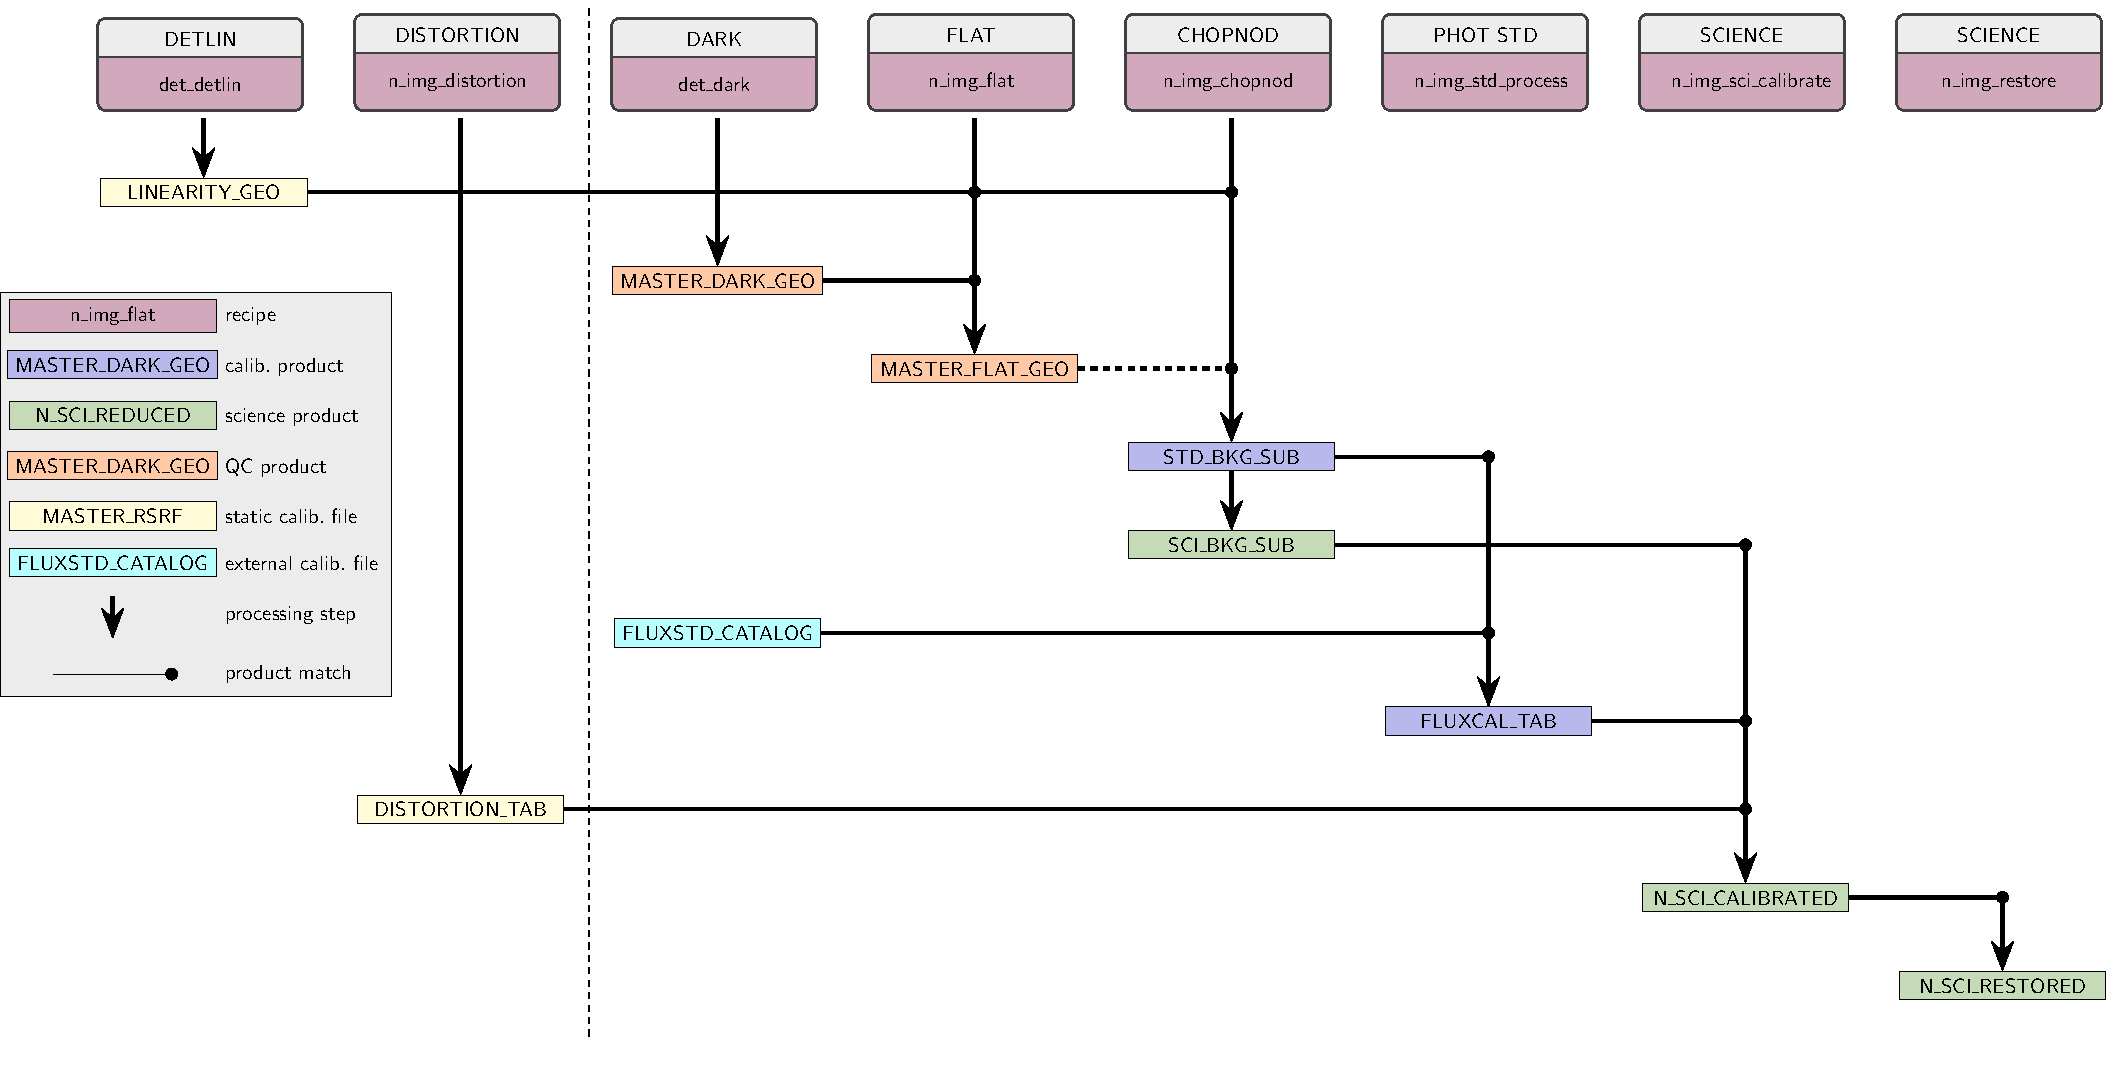
\includegraphics{IMG_N_assomap_tikz}
    \caption[Reduction cascade and association map for imaging in N]{%
      Association map for imaging in the N band. The figure shows
      only the primary product created from each recipe; for a full
      list of products refer to the recipe descriptions in
      Sect.~\ref{ssec:recipes_img_n}. The dashed line separates
      calibration tasks that are done at AIT or infrequently during
      operations (left) from daily tasks (right). The prefix ``\REC{metis_}'' has
      been omitted from the recipe names to improve clarity.}
    \label{fig:IMG_N_Assomap}
  \end{figure}
\end{landscape}

%%%%%%%%%%%%%%%%%%%%%%%%%%%%%%%%%%%%%%%%%%%%%%%%%%%%%%
%%% Local Variables:
%%% TeX-master: "METIS_DRLD"
%%% End:
